\chapter{Results}
% \textit{\ifdraft{In this section you discuss any issues that came up while developing
% the system.  If you found something particularly interesting,
% difficult, or an important learning experience, put it here.  This is
% also a good place to put additional figures and data.}}

\section{Using a robot to create image data set}\label{resrobotcontrol}
%\textbf{Robot manipulator performance was measured by making tests on two products and measuring time, iterations and interventions needed.} 
The performance of the Robot manipulator can been seen in \textit{Table \ref{tab:testonrobot}}, it has the item name, start position of the item in world-coordinates, how often the robot moved the object, how often the operator needed to interfere with the robot, time in seconds, whether the robot finished all the iterations, how long it take the robot to move one object and how often it needed intervention versus iterations. 
\vspace{1cm}
\begin{table}[h]
\resizebox{\textwidth}{!}{%
\begin{tabular}{clccccccc}
\hline
\textit{Test\#} &
  \textit{Item} &
  \textit{\begin{tabular}[c]{@{}c@{}}Start pos\\ {[}x, y, z{]}\end{tabular}} &
  \textit{Iterations} &
  \textit{\begin{tabular}[c]{@{}c@{}}Operator\\ intervention\end{tabular}} &
  \textit{\begin{tabular}[c]{@{}c@{}}Time \\ {[}sec{]}\end{tabular}} &
  \textit{\begin{tabular}[c]{@{}c@{}}Did it \\ finish?\end{tabular}} &
  \textit{\begin{tabular}[c]{@{}c@{}}Movement \\ time {[}sec{]}\end{tabular}} &
  \textit{\begin{tabular}[c]{@{}c@{}}Intervention\\ vs.  Iterations\end{tabular}} \\ \hline
\multicolumn{1}{c|}{1} &
  \begin{tabular}[c]{@{}l@{}}Nivea \\ Cleansing Milk\end{tabular} &
  \begin{tabular}[c]{@{}c@{}}{[}0.336, \\ 0.045, \\ 0.097{]}\end{tabular} &
  100 &
  2 &
  1277.2 &
  Yes &
  12.77 &
  2\% \\
\multicolumn{1}{c|}{2} &
  \begin{tabular}[c]{@{}l@{}}Alberto \\ Balsam coconut\end{tabular} &
  \begin{tabular}[c]{@{}c@{}}{[}0.343, \\ 0.043, \\ 0.107{]}\end{tabular} &
  100 &
  0 &
  1254.2 &
  Yes &
  12.54 &
  0\% \\
\multicolumn{1}{c|}{3} &
  \begin{tabular}[c]{@{}l@{}}Nivea \\ Cleansing Milk\end{tabular} &
  \begin{tabular}[c]{@{}c@{}}{[}0.340 , \\ 0.044, \\ 0.098{]}\end{tabular} &
  300 &
  6 &
  3799.1 &
  Yes &
  12.66 &
  2\%  \\
\multicolumn{1}{c|}{4} &
  \begin{tabular}[c]{@{}l@{}}Alberto \\ Balsam coconut\end{tabular} &
  \begin{tabular}[c]{@{}c@{}}{[}0.333 , \\ -0.040, \\ 0.118{]}\end{tabular} &
  300 &
  1 &
   3774.4&
  Yes &
   12.58 &
  0.33\% \\ \hline
\multicolumn{7}{r}{\textbf{Average:}} &
  12.64 &
  1.08\% \\ \hline
\end{tabular}%
}
\caption{Test made on the robot and code performance}
\label{tab:testonrobot}
\end{table}
\clearpage
%%%%%%%%%%%%%%%%%%%%%%%%%%%%%%%%%%%%%%%%%%%%%%%%%%%%%%%%%%%%%%%%%%%%%
\section{Automatic labelling}\label{rescamera}

\subsection{Before vs. after}\label{subsec:beforeafter}
\begin{figure}[ht]
    \centering
    % include first image
    \subfloat[Before]{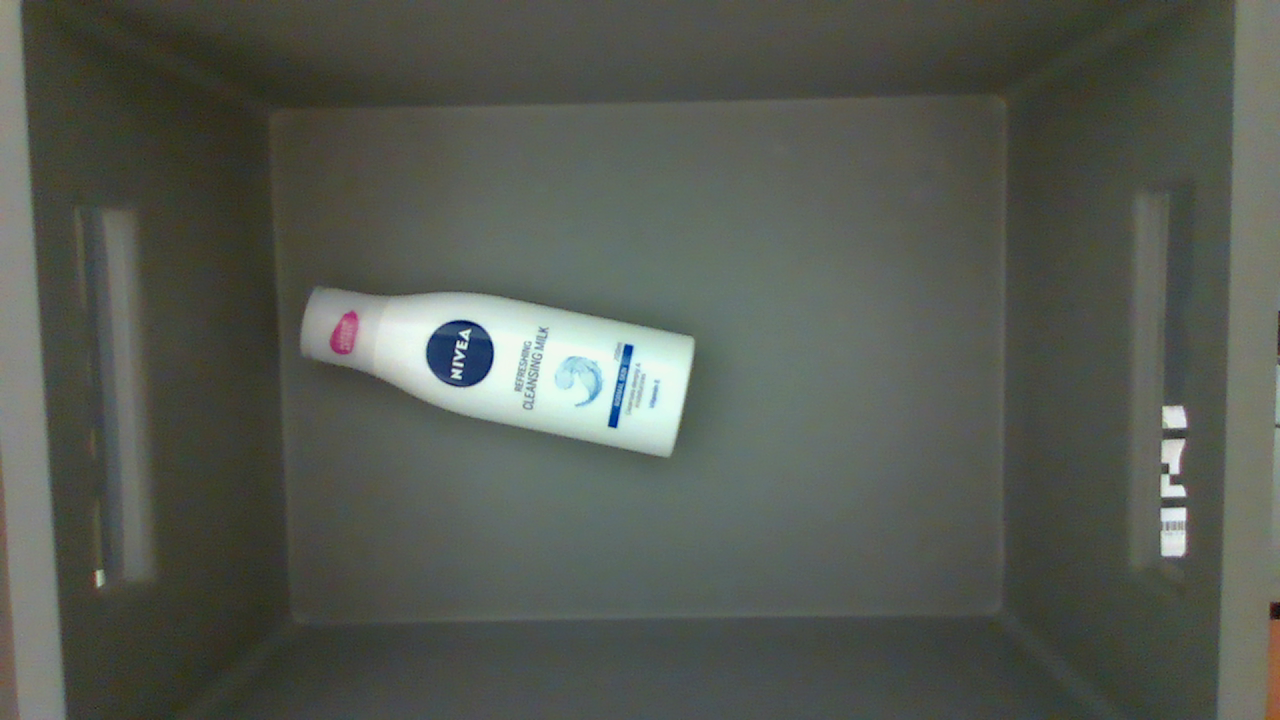
\includegraphics[width=0.495\textwidth]{graphics/9before.png}}
    \hfill
    \subfloat[After]{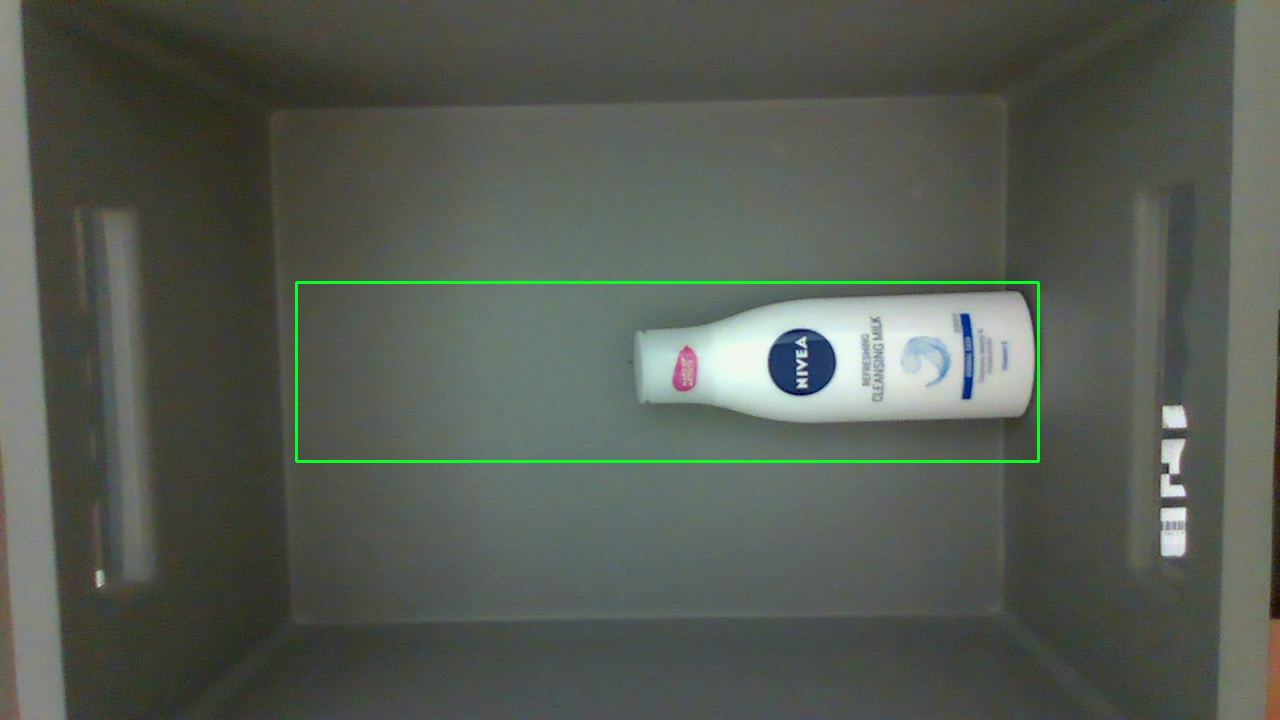
\includegraphics[width=0.495\textwidth]{graphics/9after.png}}
    \hfill
    \subfloat[Contours]{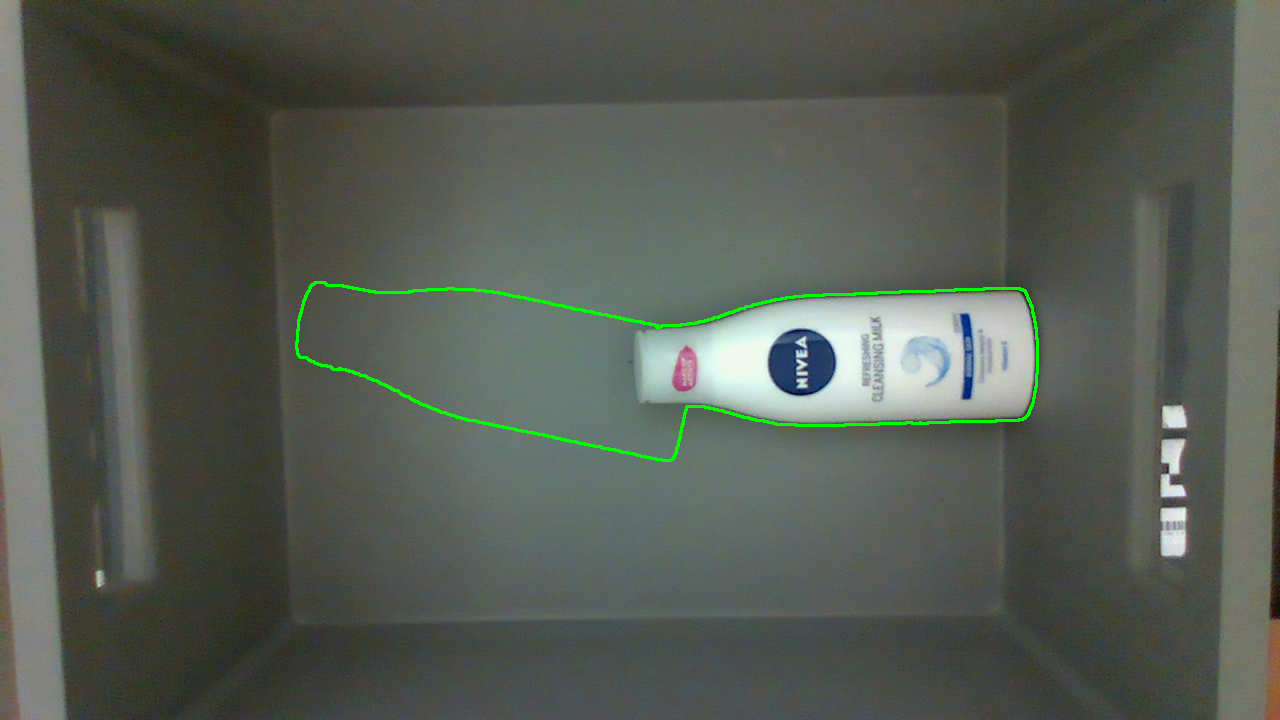
\includegraphics[width=0.495\textwidth]{graphics/9filled.png}}
    \hfill
    \subfloat[Masked]{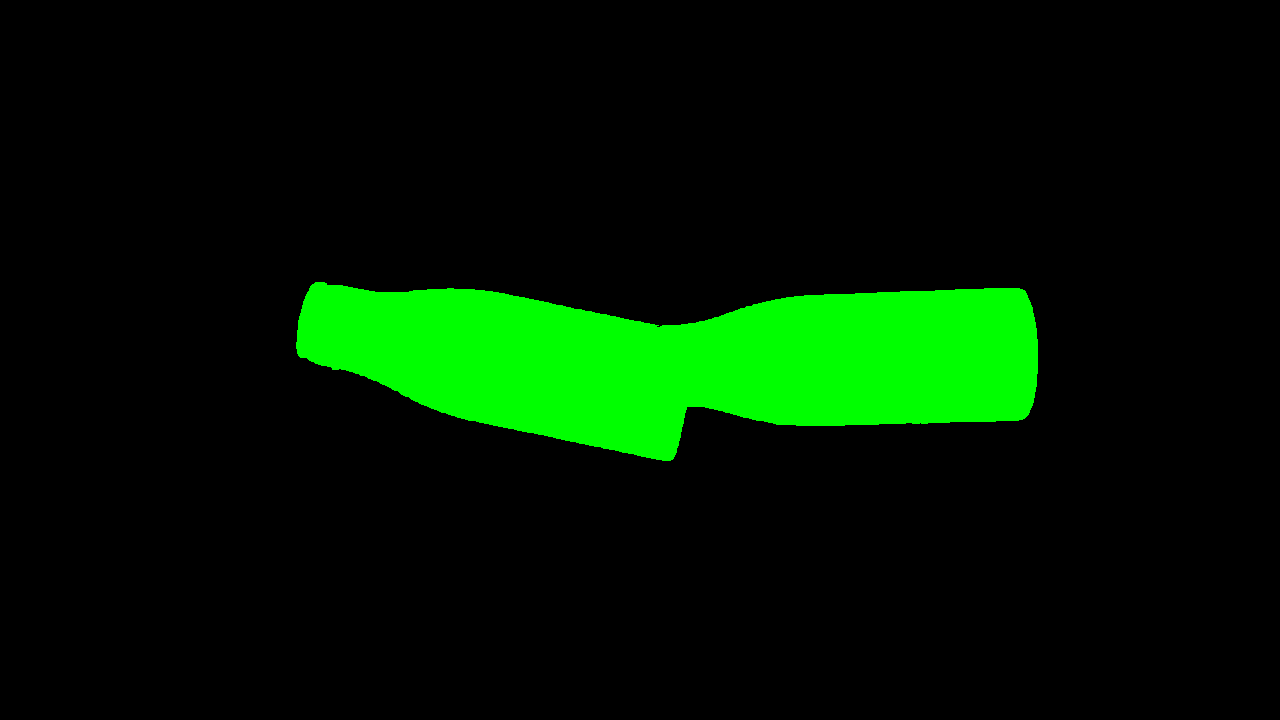
\includegraphics[width=0.495\textwidth]{graphics/9masked.png}}
    \caption{Image Difference with OpenCV and Python}
    \label{figure: imagework}
\end{figure}

In the \textit{Figure \ref{figure: imagework}} are images of the item in before position and after position. In the bottom row the contoured difference and masked contour area can be seen.  

\clearpage
\subsection{Empty bin vs. Object in the bin} \label{subsec:emptybin}
\begin{figure}[h]
    \centering
    % include first image
    \subfloat[Alberto Balsam]{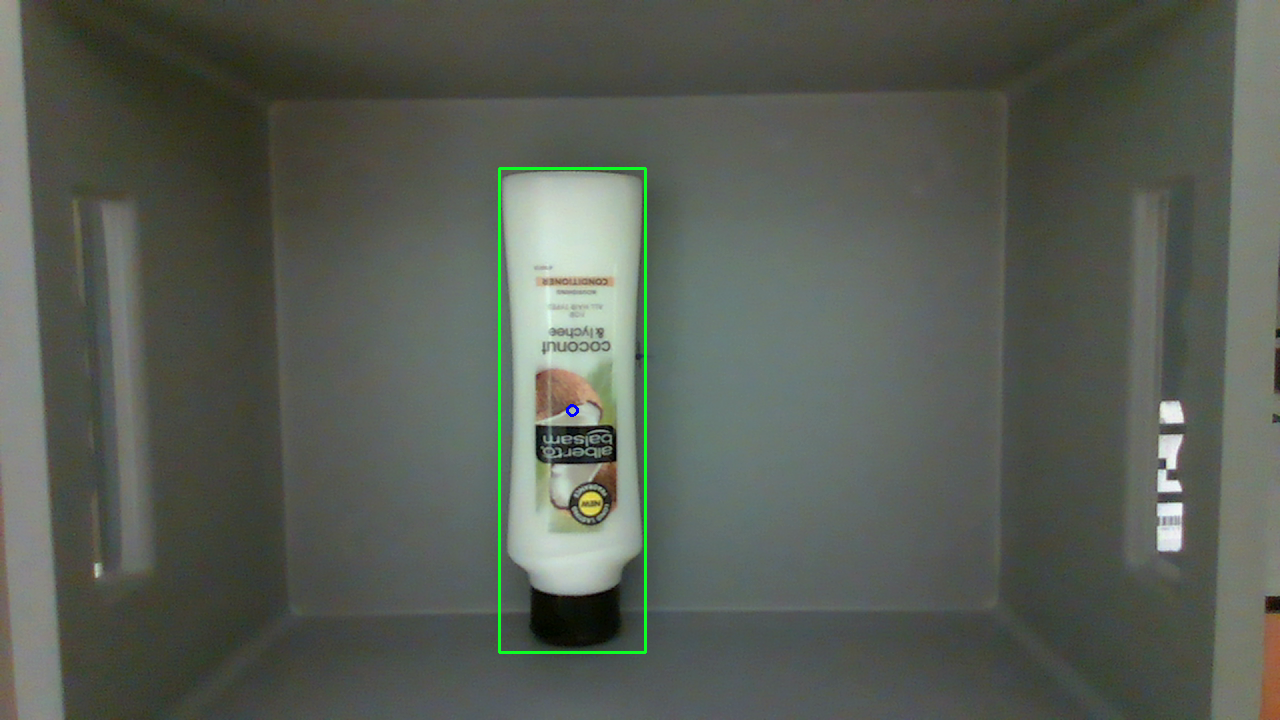
\includegraphics[width=0.495\textwidth]{graphics/results/albertobalsam100_51.png}}
    \hfill
    \subfloat[Nivea Cleansing Milk]{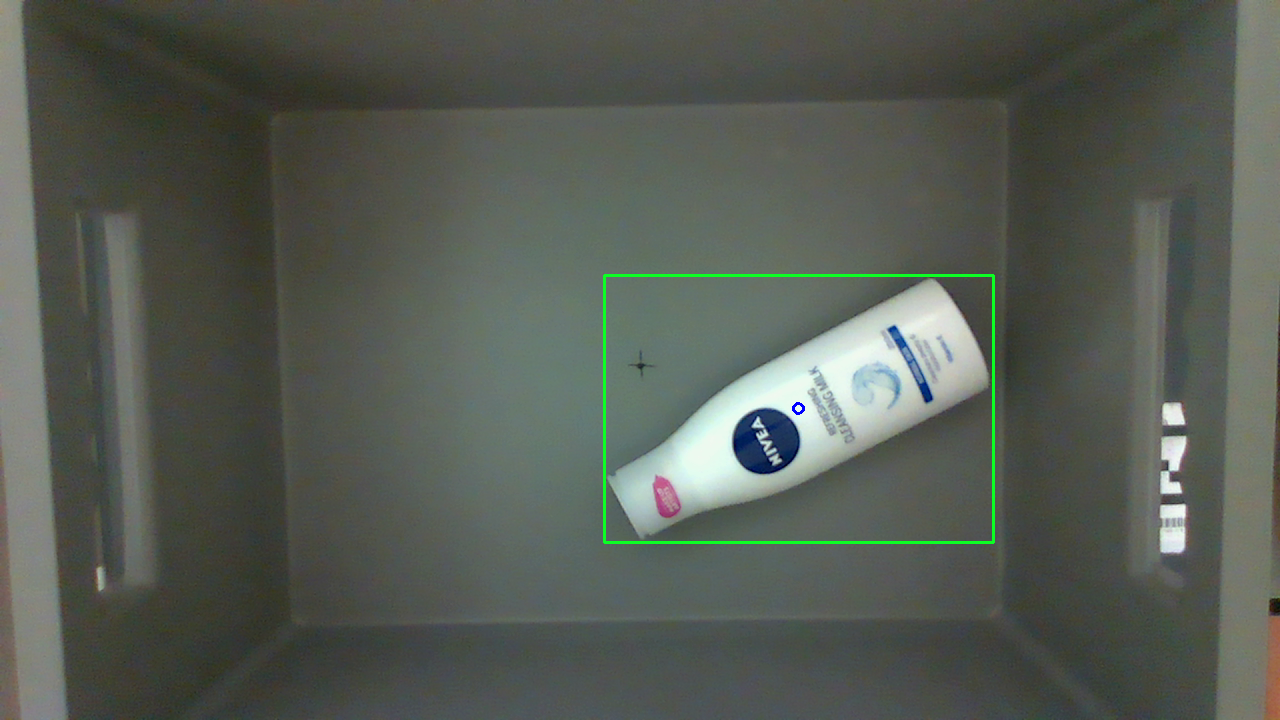
\includegraphics[width=0.495\textwidth]{graphics/results/niveacleansingmilk100_8.png}}
    \hfill
    \subfloat[Nivea Elastic]{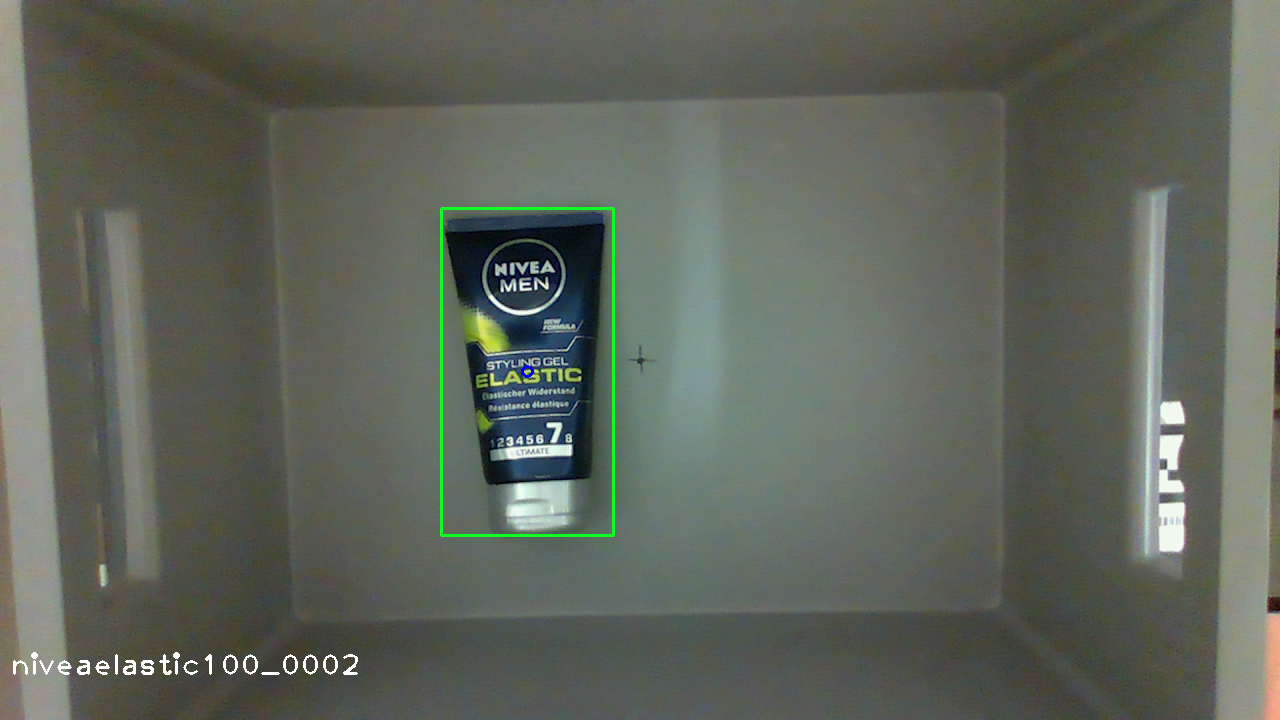
\includegraphics[width=0.495\textwidth]{graphics/results/niveaelastic100_0002box.png}}
    \hfill
    \subfloat[Nivea texture]{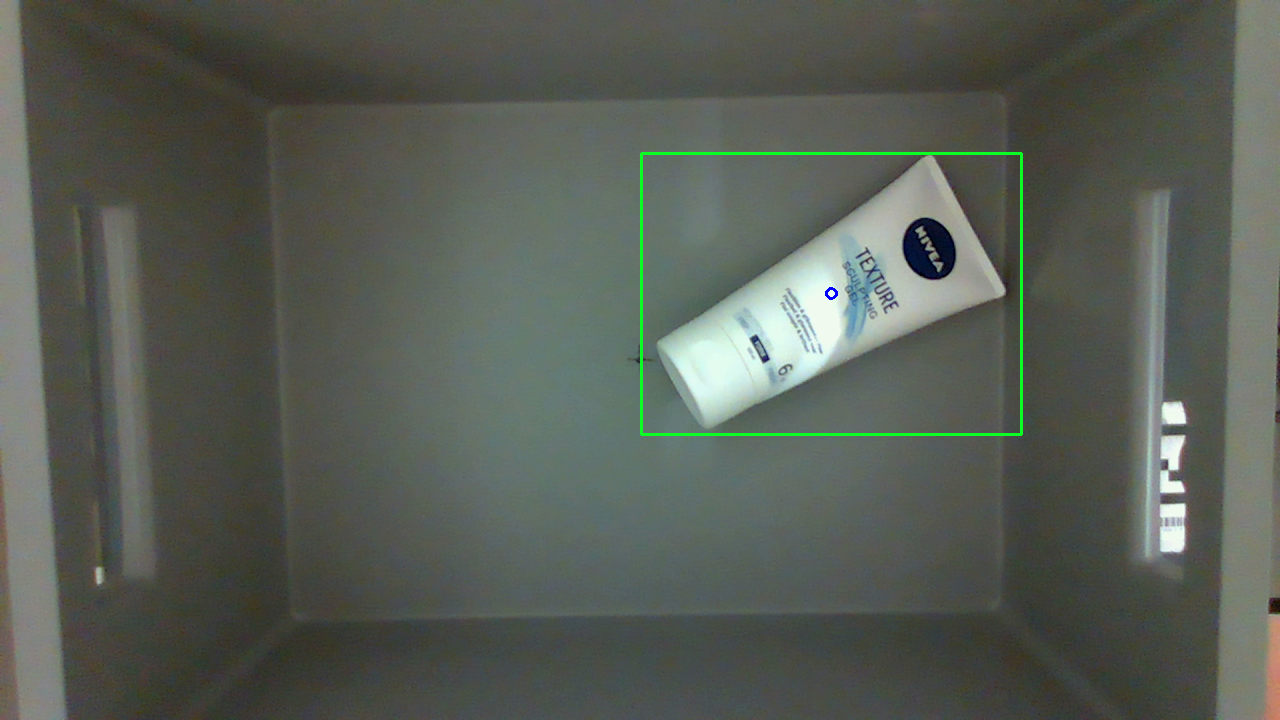
\includegraphics[width=0.495\textwidth]{graphics/results/niveatexture70_27.png}}
    \caption{The results from the difference.py, which shows the bounding box of four products}
    \label{figure: labelling}
\end{figure}
As can been seen in the \textit{Figure \ref{figure: labelling}} this method can be used to find the bounding box and to create a automatic labelled data.  
Since this method showed an increase in performance, an test was made on how long it would take to label one image. 
\textit{Table \ref{tab:timediff}} shows the results from that test. The average time to label one image is 0.85 second.
% Results from that test can been seen in \textit{Table \ref{tab:timediff}} and also it takes on average 0.85 second to label one image.



\begin{table}[h]
\resizebox{\textwidth}{!}{%
\begin{tabular}{clccc}
\hline
\multicolumn{1}{l|}{\textit{Test \#}} &
  \textit{Item} &
  \multicolumn{1}{l}{\textit{Images}} &
  \multicolumn{1}{l}{\textit{Time {[}s{]}}} &
  \multicolumn{1}{l}{\textit{Time per image {[}s{]}}} \\ \hline
\multicolumn{1}{c|}{1} & \begin{tabular}[c]{@{}l@{}}Nivea\\ cleansing milk\end{tabular}    & 300 & 255.99 & 0.85 \\
\multicolumn{1}{c|}{2} & \begin{tabular}[c]{@{}l@{}}Nivea\\ cleansing milk\end{tabular}    & 102 & 92.68  & 0.91 \\
\multicolumn{1}{c|}{3} & \begin{tabular}[c]{@{}l@{}}Nivea \\ elastic\end{tabular}          & 72  & 56.31  & 0.78 \\
\multicolumn{1}{c|}{4} & \begin{tabular}[c]{@{}l@{}}Alberto \\ Balsam coconut\end{tabular} & 102 & 88.30  & 0.87 \\ \hline
\multicolumn{4}{r}{Average:}                                                                              & 0.85
\end{tabular}%
}
\caption{Measured time when using the difference.py}
\label{tab:timediff}
\end{table}

\clearpage
%%%%%%%%%%%%%%%%%%%%%%%%%%%%%%%%%%%%%%%%%%%%%%%%%%%%%%%%%%%%%%%%%%%%%
\section{Results from the first neural network}
\begin{figure}[h]
    \centering
    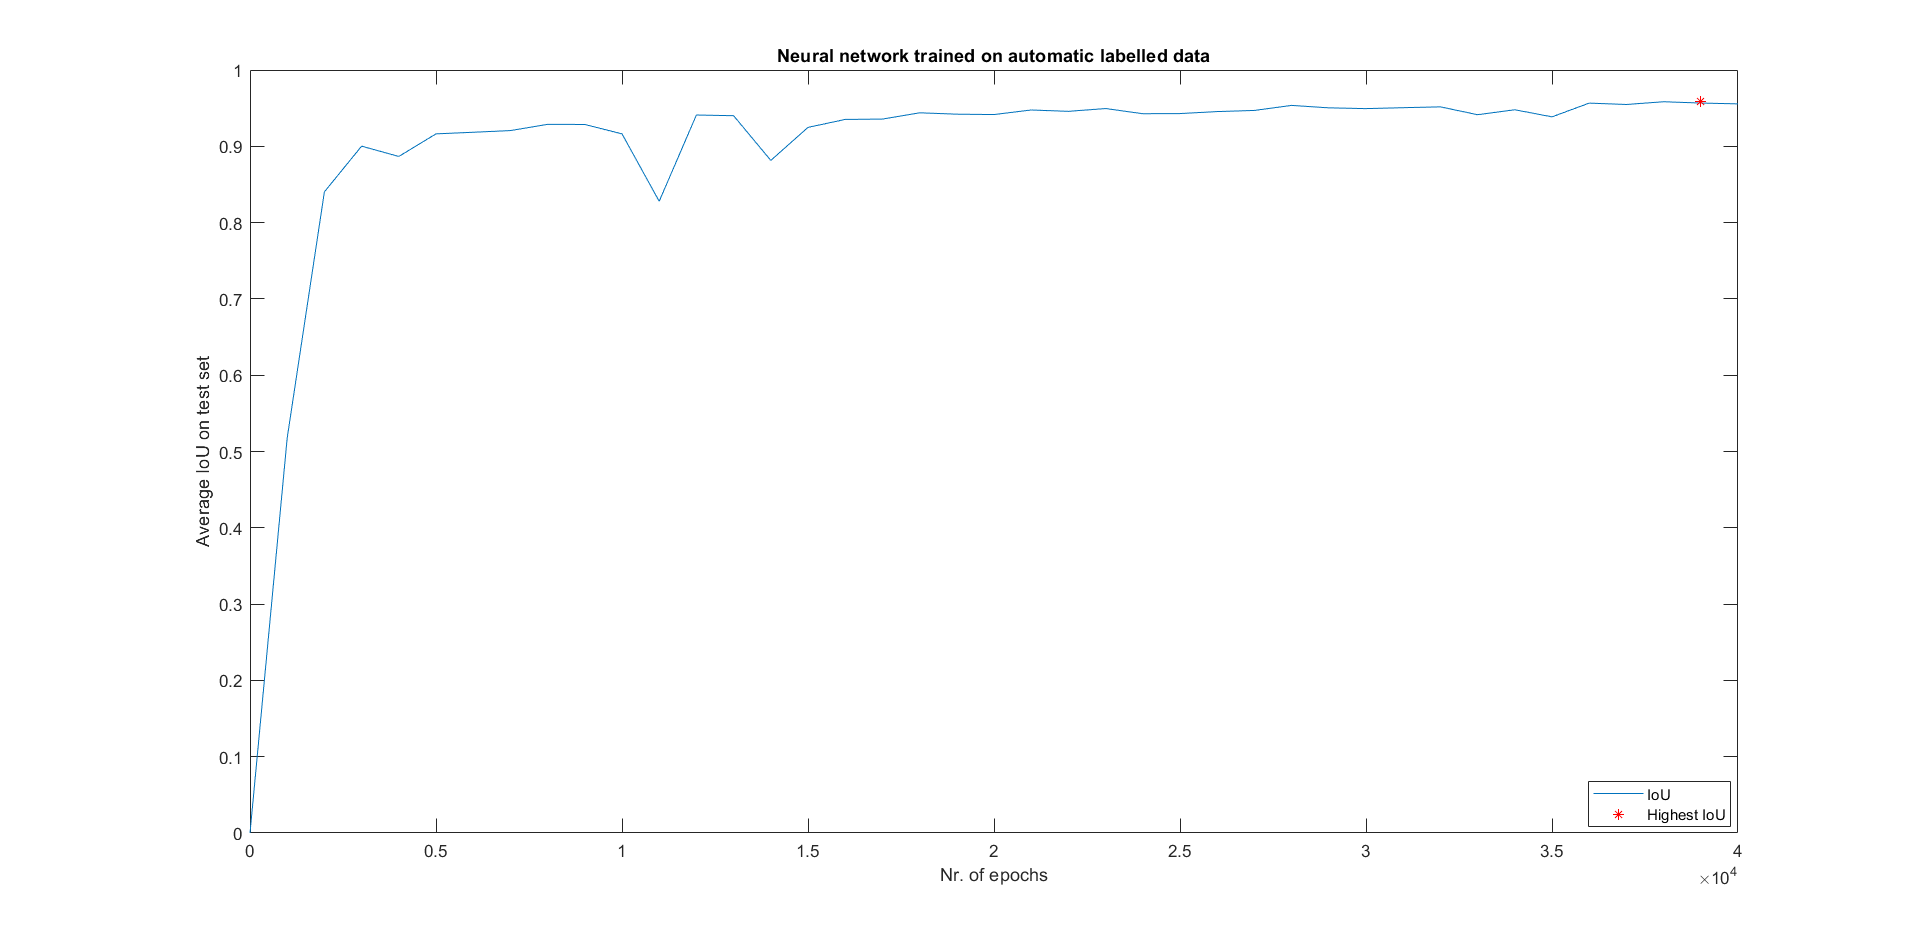
\includegraphics[width=0.8\textwidth, trim={5cm 0 4cm 0},clip]{graphics/results/neuralnetworkauto.png}
    \caption{IoU every 1000 epochs}
    \label{fig:neuralnetwork}
\end{figure}
\textit{Figure \ref{fig:neuralnetwork}} shows how the IoU score developed over the number of epochs. The best average IoU score can be seen in the red point and is 0.9584 at 39000 epochs. The average IoU is measured when running through the test dataset.

\begin{figure}[h]
    \centering
    % include first image
    \subfloat[Using YOLOv4]{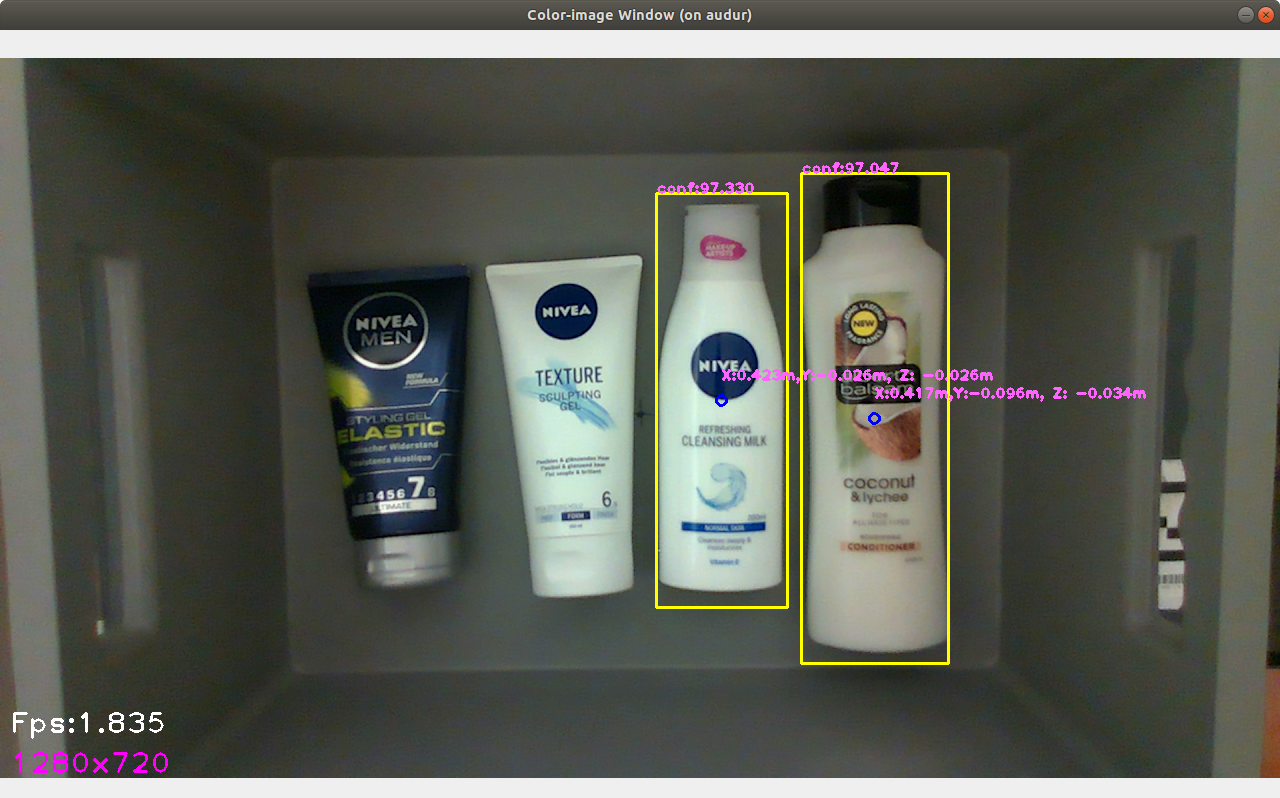
\includegraphics[width=0.33\textwidth, trim={0 0.6cm 0 2cm},clip ]{graphics/results/beforetraining.png}}
    \hfill
    \subfloat[Using YOLOv4]{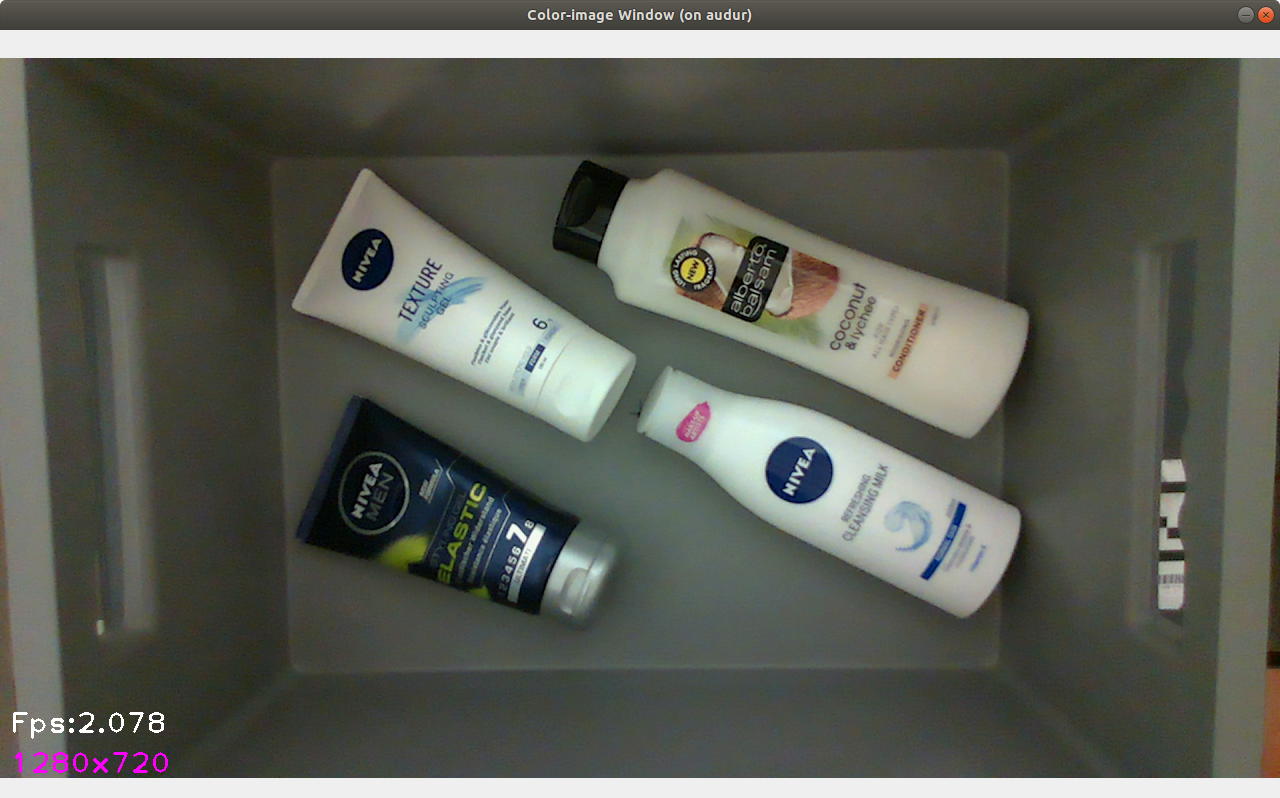
\includegraphics[width=0.33\textwidth, trim={0 0.6cm 0 2cm},clip]{graphics/results/beforetraining1.png}}
    \hfill
    \subfloat[Using YOLOv4]{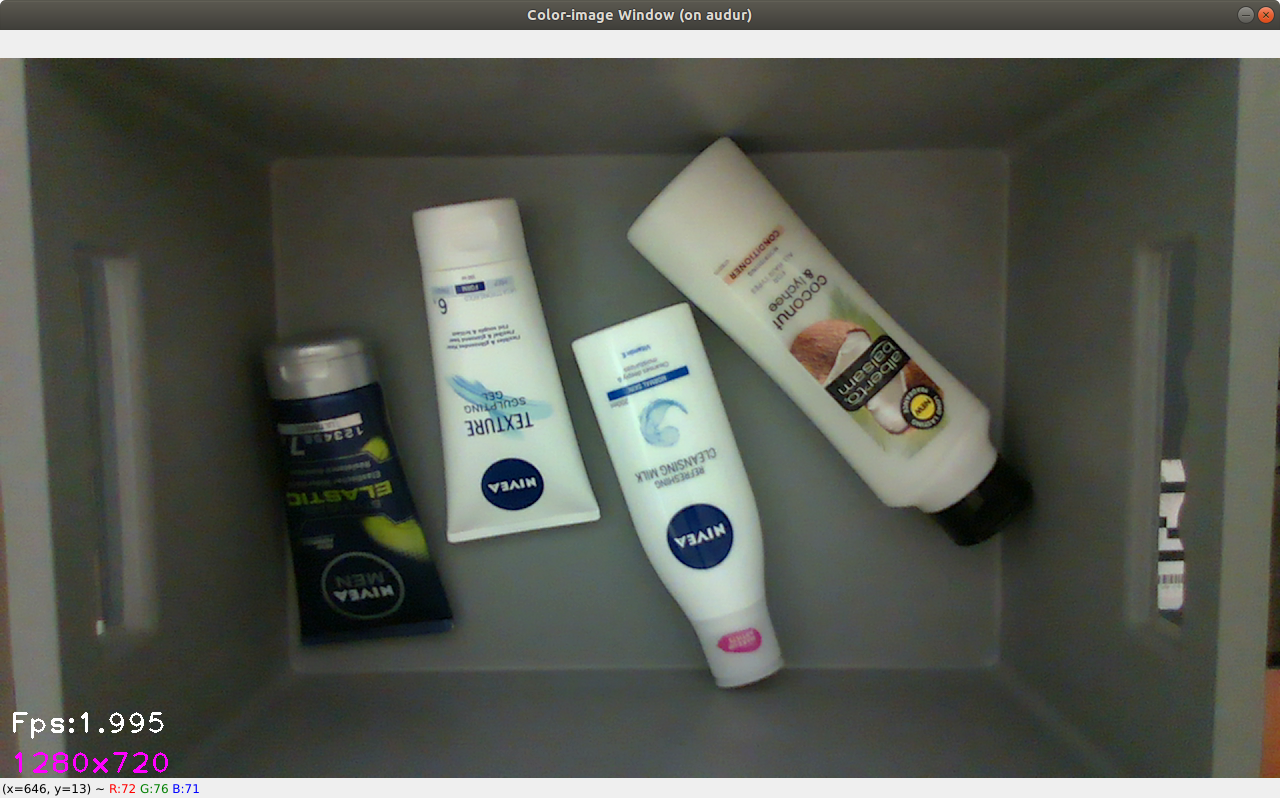
\includegraphics[width=0.33\textwidth, trim={0 0.6cm 0 2cm},clip]{graphics/results/beforetraining2.png}}
    \hfill
    \subfloat[Using trained YOLOv4]{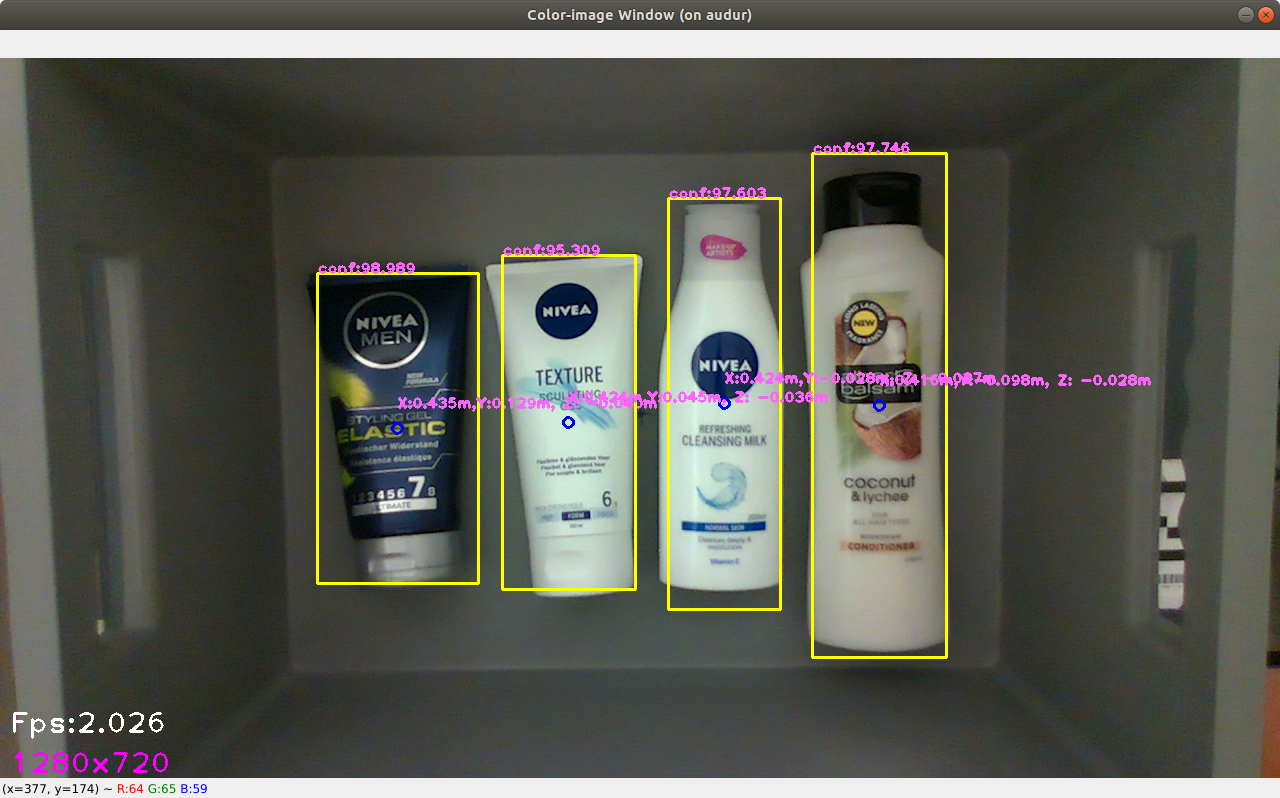
\includegraphics[width=0.33\textwidth, trim={0 0.6cm 0 2cm},clip]{graphics/results/aftertraining.png}}
    \hfill
    \subfloat[Using trained YOLOv4]{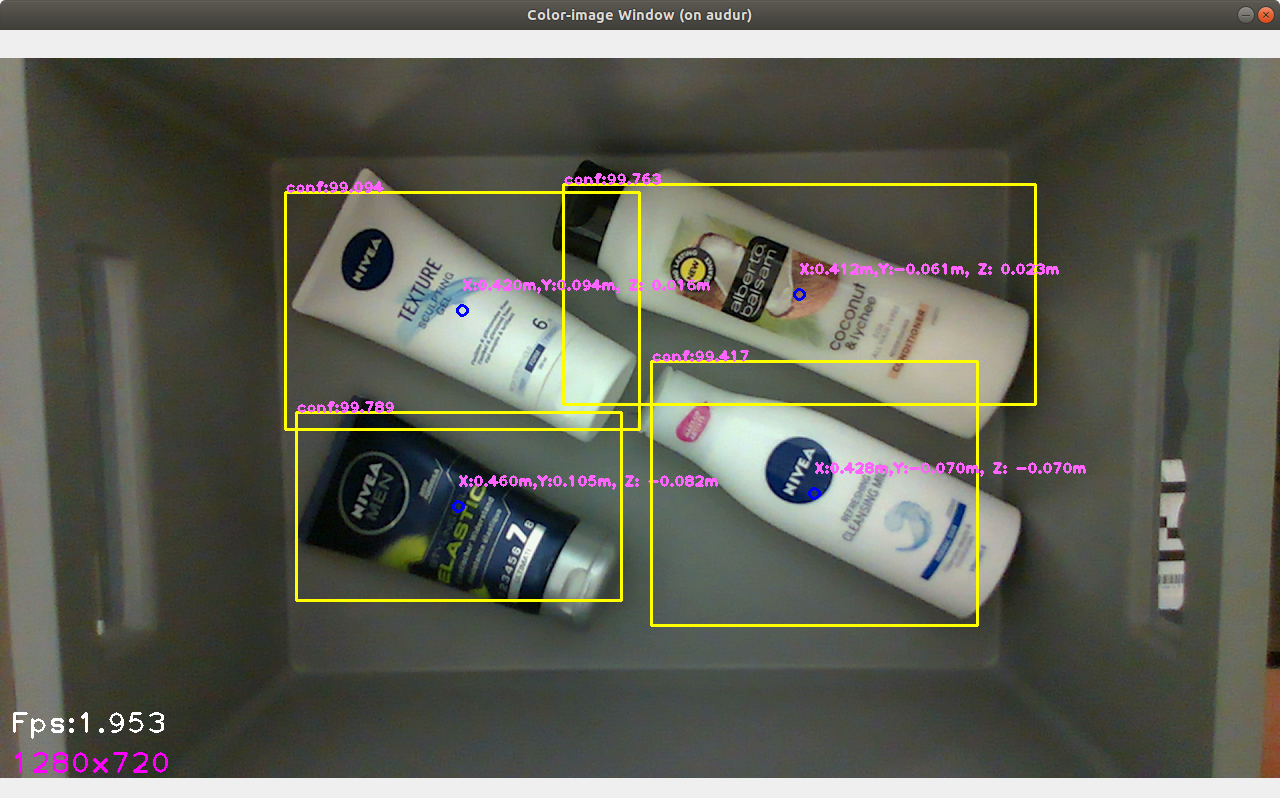
\includegraphics[width=0.33\textwidth, trim={0 0.6cm 0 2cm},clip]{graphics/results/aftertraining1.png}}
    \hfill
    \subfloat[Using trained YOLOv4]{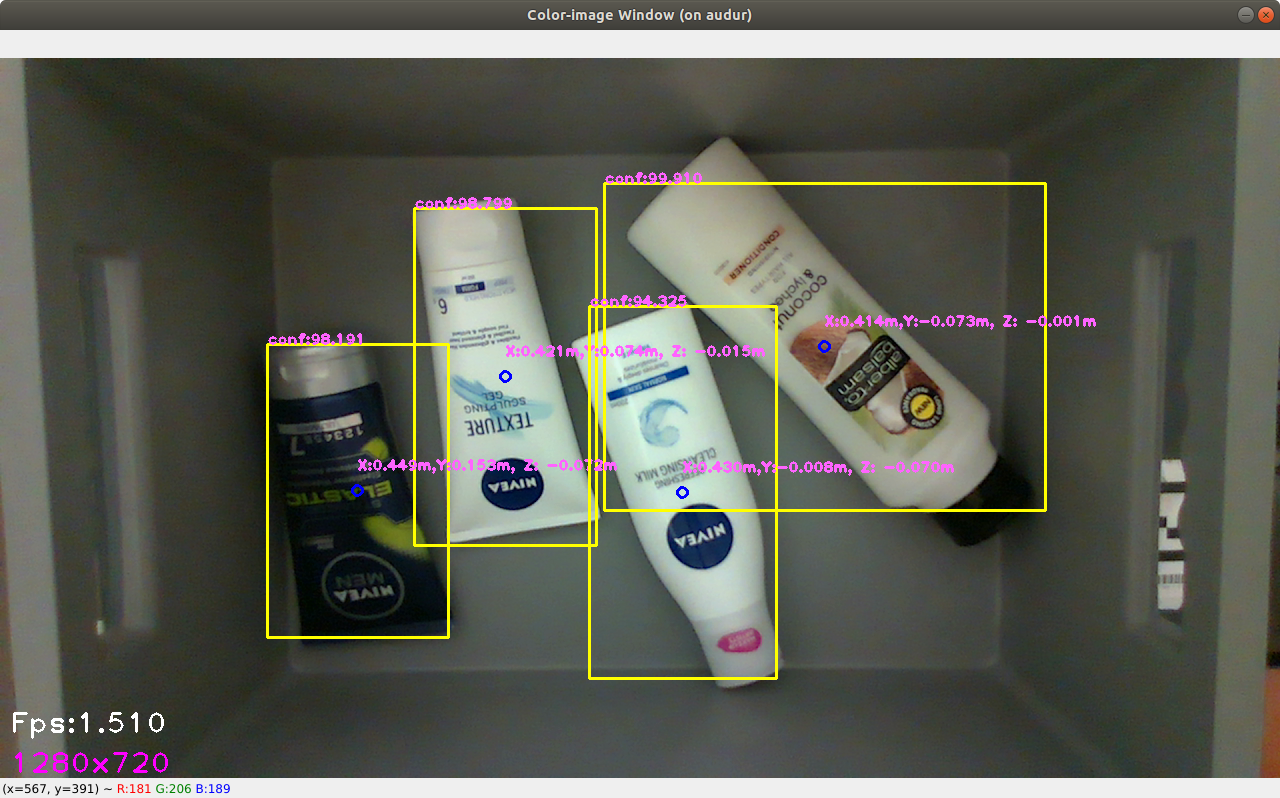
\includegraphics[width=0.33\textwidth, trim={0 0.6cm 0 2cm},clip]{graphics/results/aftertraining2.png}}
    \caption{Using YOLOv4 and the trained YOLOv4 model, trained on images from the robot}
    \label{figure: beforeaftertraining}
\end{figure}
\textit{Figure \ref{figure: beforeaftertraining}} shows visually how the performance changed before and after training, images in top row shows the results from YOLOv4 and images in the bottom row shows the results from a trained YOLOv4 that was trained on these products.

\pagebreak
\subsection{On trained items}\label{sec:resontrained}
\begin{figure}[h]
    \centering
    % include first image
    \subfloat[Alberto Balsam]{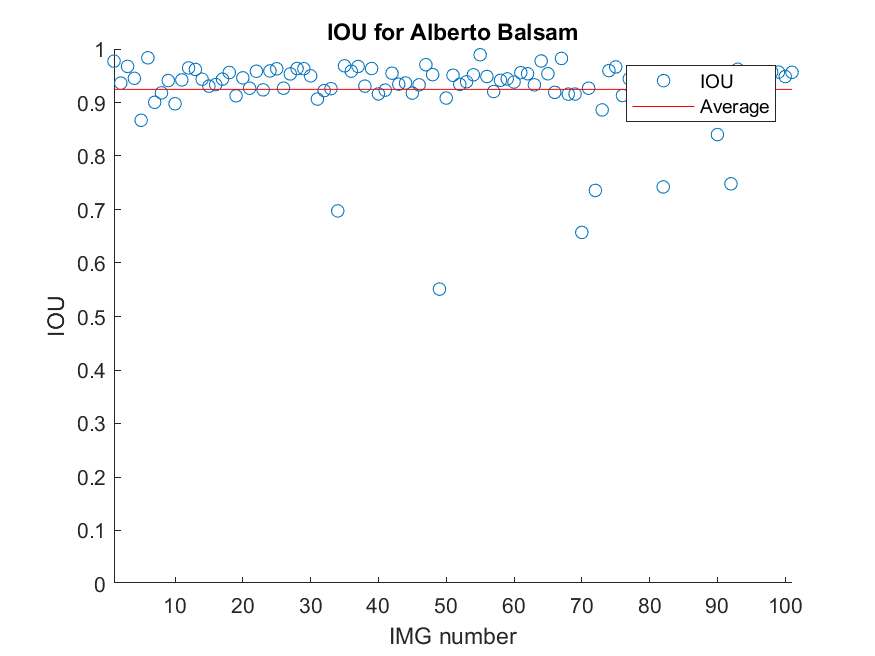
\includegraphics[width=0.485\textwidth, trim={0.6cm 0 0.6cm 0},clip]{graphics/albertobalsamIOU.png}}
    \hfill
    \subfloat[Nivea Cleansing Milk]{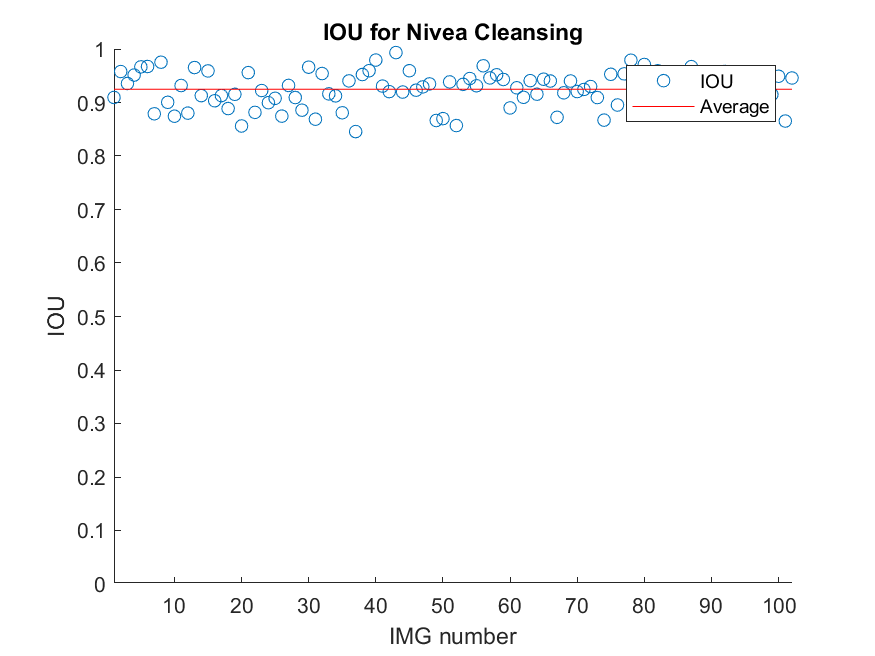
\includegraphics[width=0.485\textwidth, trim={0.6cm 0 0.6cm 0},clip]{graphics/niveacleansingIOU.png}}
    \hfill
    \subfloat[Nivea Elastic]{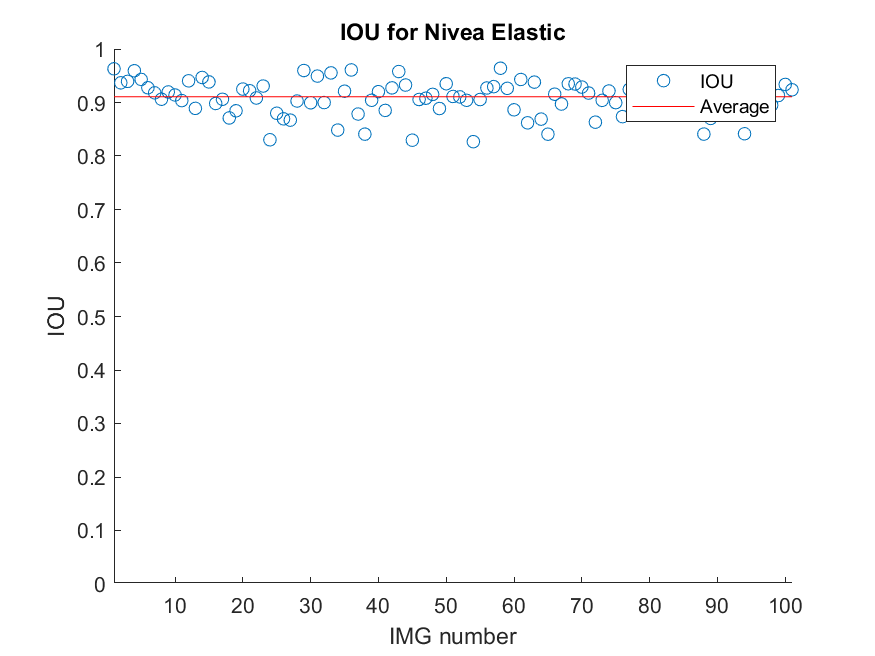
\includegraphics[width=0.485\textwidth, trim={0.6cm 0 0.6cm 0},clip]{graphics/niveaelasticIOU.png}}
    \hfill
    \subfloat[Nivea Texture]{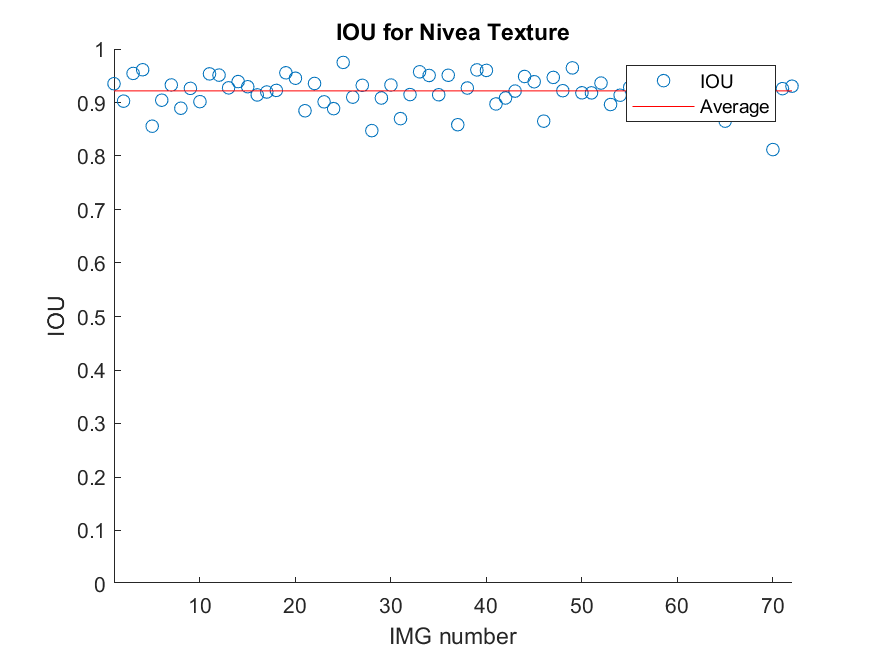
\includegraphics[width=0.485\textwidth, trim={0.6cm 0 0.6cm 0},clip]{graphics/niveatextureIOU.png}}
    \caption{Scatter plot for IoU on known products}
    \label{figure: knownproducts}
\end{figure}
\textit{Figure \ref{figure: knownproducts}} shows raw IoU data from detection run on the first dataset \textit{(Sec: \ref{sec:firstdataset})}, it also shows an average IoU line on each scatter plot.

\begin{table}[h]
\resizebox{\textwidth}{!}{% 
\begin{tabular}{l|cccccccc}
\hline
\textit{Item} &
  \textit{Products} &
  \textit{Detections} &
  \textit{True Positive} &
  \textit{False Positive} &
  \textit{Avg-IoU} &
  \textit{Avg-Precision} &
  \textit{Avg-Recall} &
  \textit{Avg-F1} \\ \hline
Alberto Balsam & 101 & 101 & 101 & 0 & 0.9244 & 1 & 1 & 1 \\
Nivea C. Milk & 102 & 102 & 102 & 0 & 0.9248 & 1 & 1 & 1 \\
Nivea Elastic & 101 & 101 & 101 & 0 & 0.9107 & 1 & 1 & 1 \\
Nivea Texture & 72  & 72  & 72  & 0 & 0.9217 & 1 & 1 & 1 \\ \hline
\end{tabular}%
}
\caption{Detection results when tested on trained data}
\label{tab:ready}
\end{table}
\textit{Table \ref{tab:ready}} shows the results from the detection run on the first dataset \textit{(Sec: \ref{sec:firstdataset})} when using the trained YOLOv4 network on known products.

\begin{figure}[h]
    \centering
    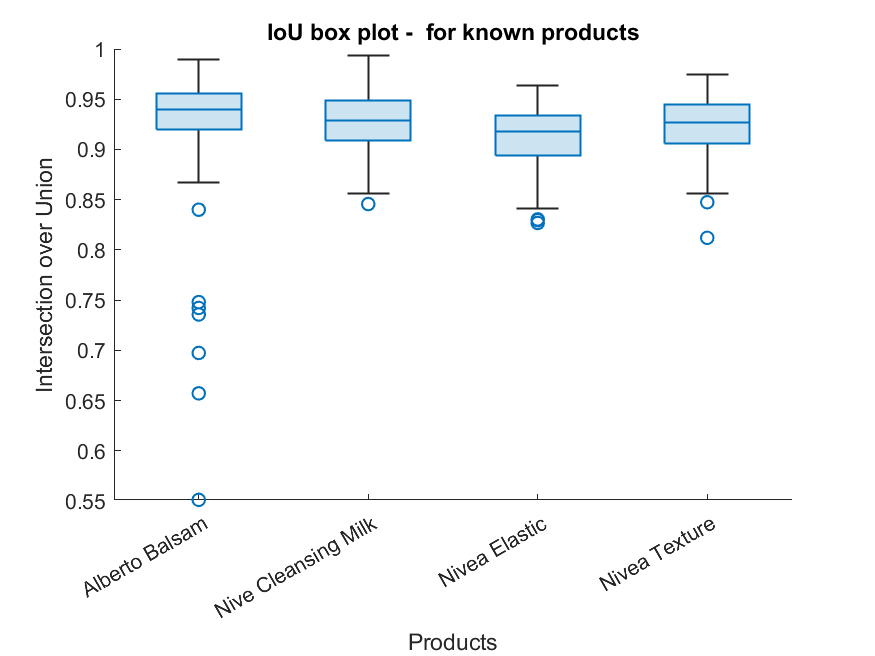
\includegraphics[width=0.9\textwidth]{graphics/results/boxplotForKnownProducts.png}
    \caption{Box plot for known products}
    \label{fig:boxknownproducts}
\end{figure}
\textit{Figure \ref{fig:boxknownproducts}} shows the IoU on 4 known products in a box plot. The ends of the box are the upper and lower quartiles,  the vertical line inside the box is the median, and the bottom and top line is a lower extreme and upper extreme.



\clearpage
\subsection{On unknown Beiersdorf products}\label{subsec:resunknownprod}
\begin{figure}[h]
    \centering
    % include first image
    \subfloat[Item 11]{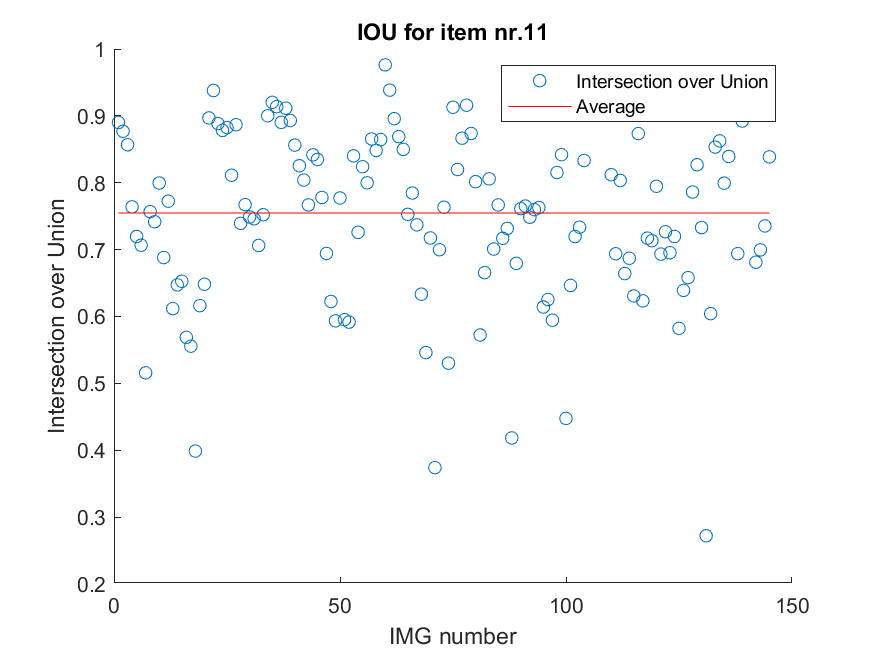
\includegraphics[width=0.5\textwidth, trim={0.6cm 0 0.6cm 0},clip]{graphics/results/item11.png}}
    \hfill
    % \subfloat[Item 12]{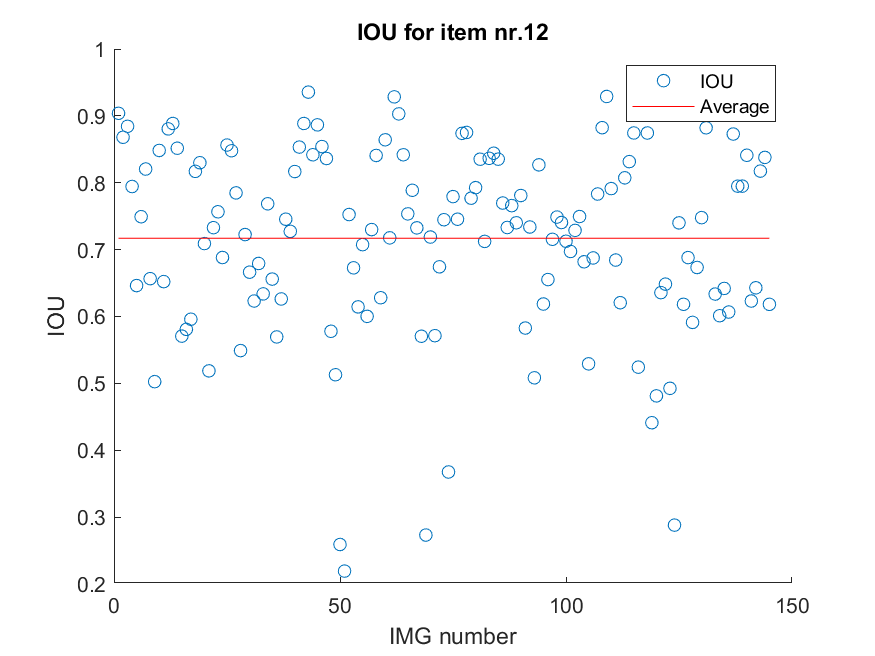
\includegraphics[width=0.245\textwidth]{graphics/results/item12.png}}
    % \hfill
    % \subfloat[Item 5]{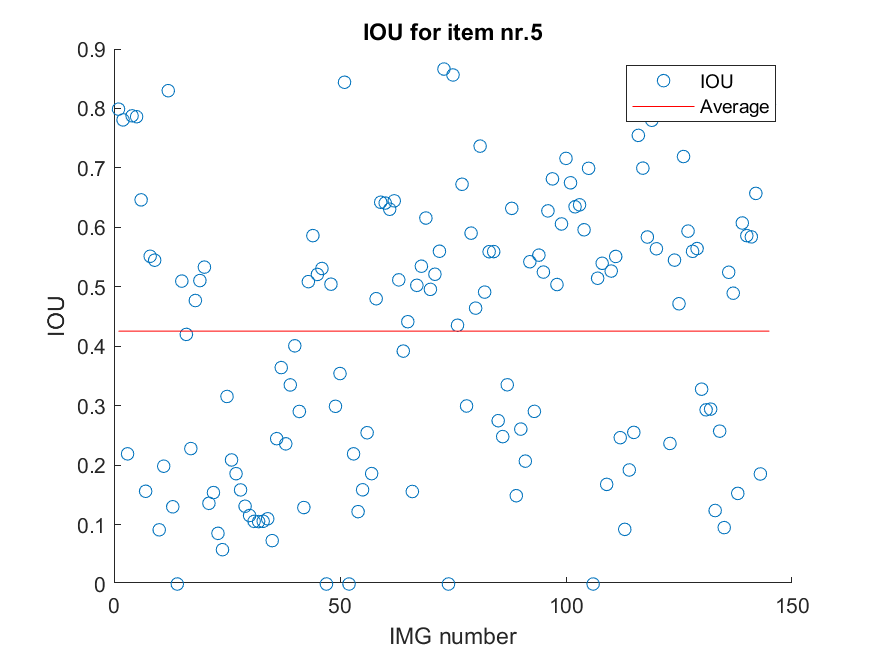
\includegraphics[width=0.245\textwidth]{graphics/results/item5.png}}
    % \hfill
    \subfloat[Item 6]{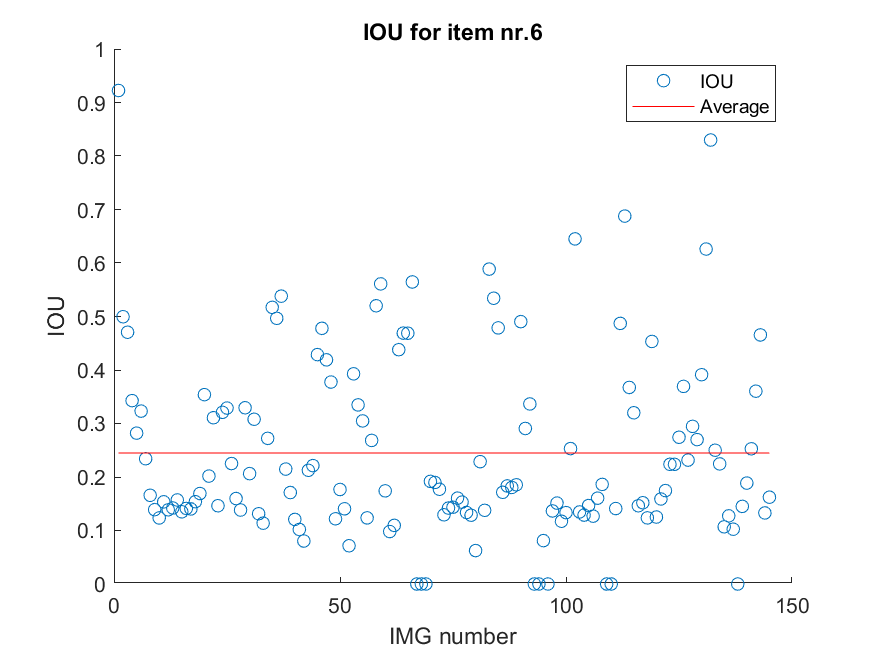
\includegraphics[width=0.5\textwidth, trim={0.6cm 0 0.6cm 0},clip]{graphics/results/item6.png}}
    \caption{Scatter plot for IoU on unknown products}
    \label{figure: unknownproducts}
\end{figure}

\textit{Figure \ref{figure: unknownproducts}} shows raw IoU data from detection run on the Beiersdorf dataset \textit{(Sec: \ref{sec:beiersdorfdataset})}, it also shows an average IoU line on each scatter plot. 
Item nr. 11 had the highest average IoU or 0.725 and item nr. 6 had the lowest average IoU or 0.245. Raw data can be seen in the \textit{Appendix \ref{sec:IoUresult}}.
\begin{table}[h]
\resizebox{\textwidth}{!}{%
\begin{tabular}{c|cccccccc}
\hline
\textit{Item} &
  \textit{Products} &
  \textit{Detections} &
  \textit{True Positive} &
  \textit{False Positive} &
  \textit{Avg-IoU} &
  \textit{Avg-Precision} &
  \textit{Avg-Recall} &
  \textit{Avg-F1} \\ \hline
1  & 684  & 332 & 300 & 29  & 0.648  & 0.8299 & 0.5032 & 0.595  \\
2  & 1029 & 392 & 330 & 55  & 0.579  & 0.7327 & 0.3862 & 0.471  \\
3  & 667  & 368 & 337 & 29  & 0.6734 & 0.8523 & 0.569  & 0.6542 \\
4  & 683  & 350 & 325 & 24  & 0.7058 & 0.8891 & 0.5426 & 0.6394 \\
5  & 892  & 317 & 202 & 110 & 0.4253 & 0.5205 & 0.2418 & 0.3194 \\
6  & 918  & 195 & 57  & 129 & 0.2449 & 0.1833 & 0.0682 & 0.0956 \\
7  & 851  & 405 & 326 & 78  & 0.5757 & 0.7314 & 0.3907 & 0.4956 \\
8  & 788  & 292 & 264 & 26  & 0.664  & 0.8615 & 0.3707 & 0.4895 \\
9  & 887  & 333 & 270 & 60  & 0.536  & 0.7218 & 0.3308 & 0.4349 \\
10 & 665  & 344 & 293 & 51  & 0.626  & 0.7736 & 0.4761 & 0.5667 \\
11 & 627  & 385 & 361 & 23  & 0.7245 & 0.8994 & 0.623  & 0.7106 \\
12 & 574  & 417 & 394 & 23  & 0.7171 & 0.9268 & 0.7376 & 0.7971 \\
13 & 618  & 307 & 291 & 14  & 0.694  & 0.9149 & 0.5309 & 0.6403 \\
14 & 1031 & 245 & 180 & 52  & 0.5178 & 0.6299 & 0.2211 & 0.3012 \\
15 & 616  & 302 & 273 & 23  & 0.6897 & 0.8368 & 0.4918 & 0.5858 \\ 
\hline
\end{tabular}%
}
\caption{The results when tested on unknown data}
\label{tab:test1unknown}
\end{table}

\textit{Table \ref{tab:test1unknown}} shows the results from the detection run on the Beiersdorf dataset \textit{(Sec: \ref{sec:beiersdorfdataset})} when using the trained YOLOv4 network on unknown products. As can be seen item nr. 12 has the best average precision, recall and F-score.

% \begin{figure}[h]
%     \centering
%     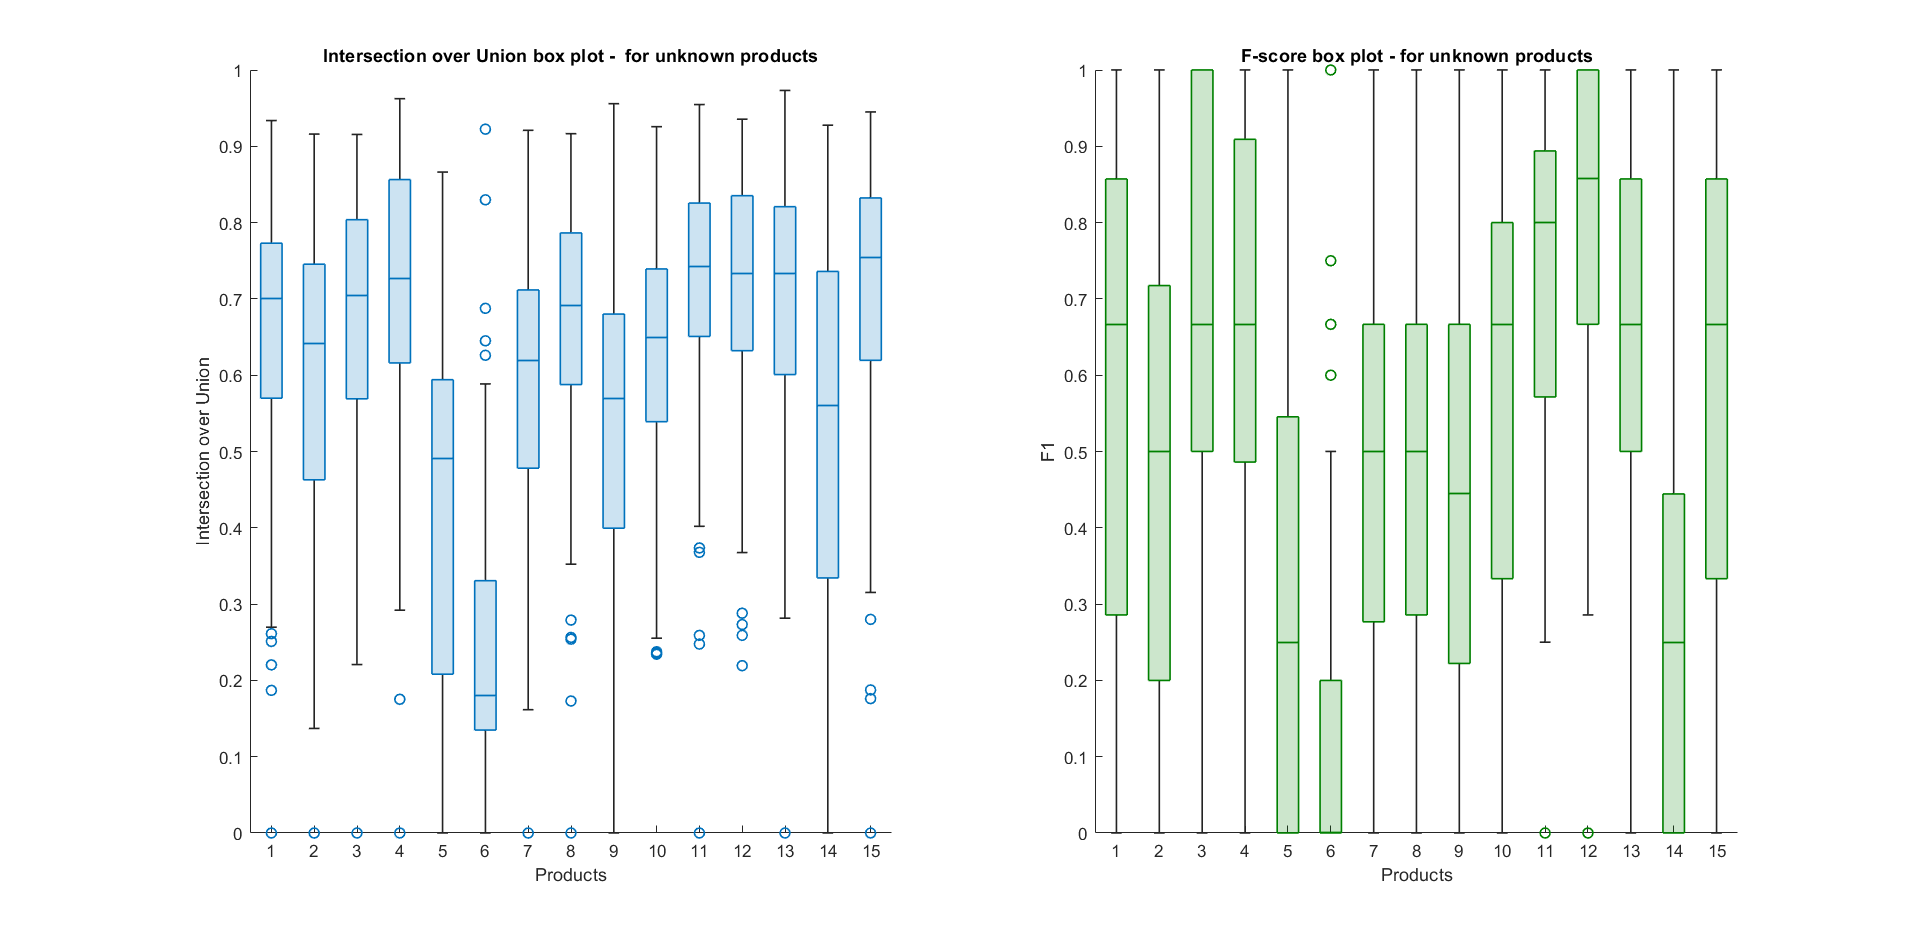
\includegraphics[width=1\textwidth, trim={8cm 0 8cm 0},clip]{graphics/results/boxplotForProducts.png}
%     \caption{Box plot for unknown products, Intersection over Union on the left and F-score on the right}
%     \label{fig:boxunknownproducts}
% \end{figure}
\clearpage

\begin{figure}[h]
    \centering
    % include first image
    \subfloat[Intersection over Union]{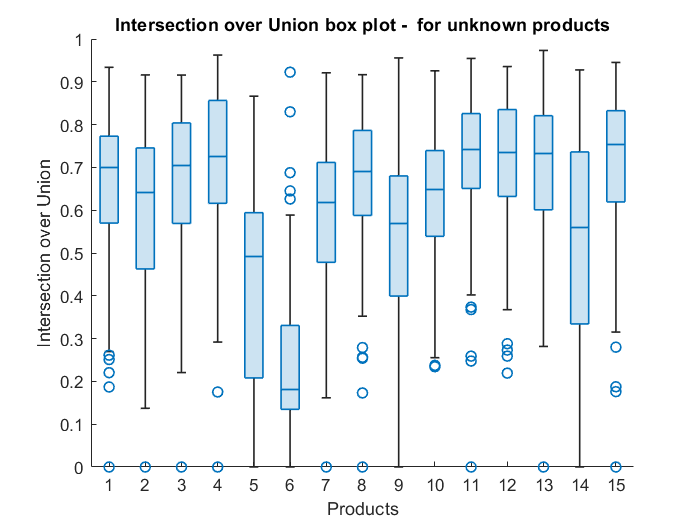
\includegraphics[width=0.5\textwidth, trim={1cm 0 1.5cm 0},clip]{graphics/results/boxplotForProducts2.png}\label{fig:unknownioua}}
    \hfill
    \subfloat[F-score]{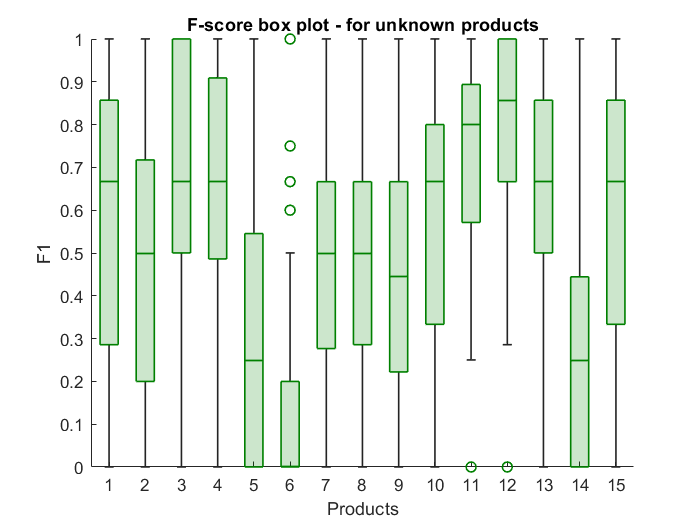
\includegraphics[width=0.5\textwidth, trim={1cm 0 1.5cm 0},clip]{graphics/results/boxplotForProducts1.png}\label{fig:unknownioub}}
    
    \caption{Box plot on results for unknown products}
    \label{fig:unknowniou}
\end{figure}

\textit{Figure \ref{fig:unknowniou}} shows the IoU and F-score on 15 unknown products in a box plot.
\begin{figure}[h]
    \centering
    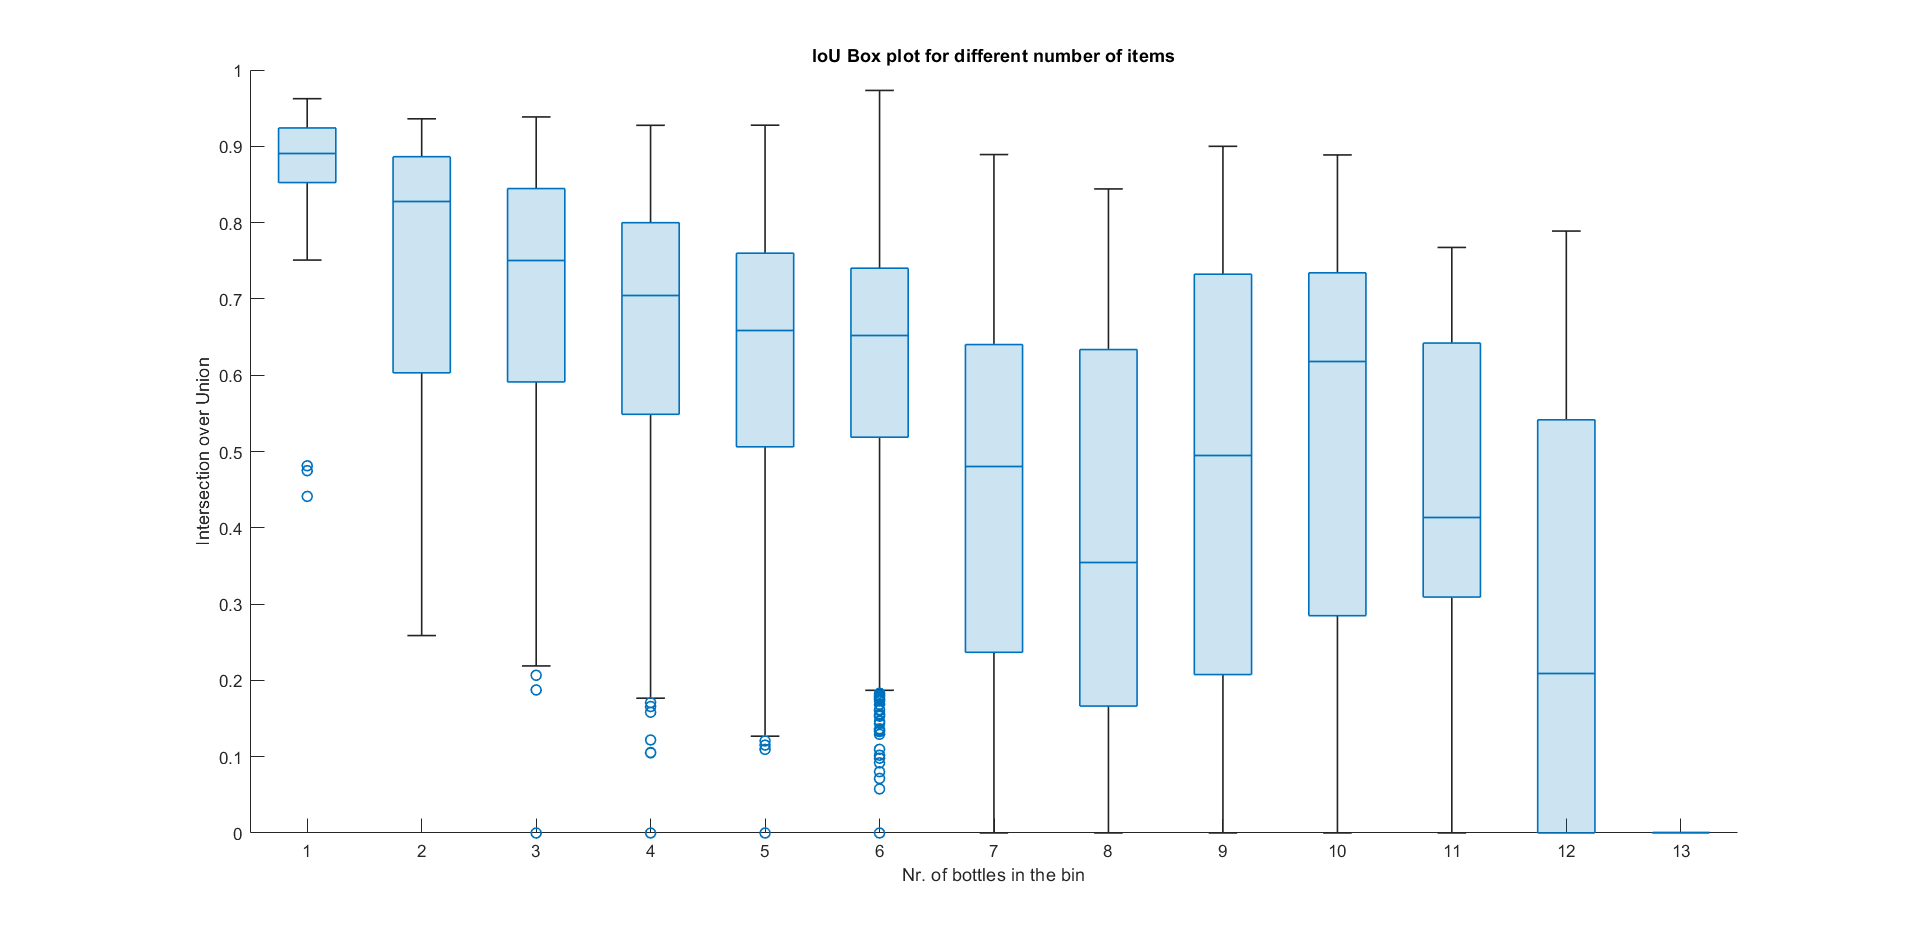
\includegraphics[width=1\textwidth]{graphics/results/boxplotBottles.png}
    \caption{IoU box plot for different number of items}
    \label{fig:bottles}
\end{figure}

\textit{Figure \ref{fig:bottles}} shows also the IoU in box plot, but for different number of objects in the bin.